\documentclass[mathserif]{beamer}
\usepackage{amsmath}
\usepackage{tikz}

\title{Ultrafast and memory-efficient alignment of short DNA sequences
to the human genome}
\subtitle{\textit{Ben Langmead, Cole Trapnell, \\Mihai Pop and Steven L Salzberg}}

\author{Akshay Sanjeev}


\begin{document}
\begin{frame}
    \maketitle
\end{frame}


\begin{frame}{We are in 2009}

\end{frame}

\begin{frame}{Outline of Bowtie}
    \begin{itemize}
        \item Burrows-Wheeler Transform(Indexing)
        \item Exact and inexact alignment
        \item Excessive backtracking
    \end{itemize}
\end{frame}


\begin{frame}{Burrows- Wheeler Transform: Forward Transform}
    Let $T=\texttt{BANANA}$. BWT$(T)$ will be:
    \[
    \begin{bmatrix}
        \texttt{\$} &\texttt{B} &\texttt{A} &\texttt{N} &\texttt{A} &\texttt{N} &\texttt{A} \\
        \texttt{A} &\texttt{\$} &\texttt{B} &\texttt{A} &\texttt{N} &\texttt{A} &\texttt{N} \\
        \texttt{N} &\texttt{A} &\texttt{\$} &\texttt{B} &\texttt{A} &\texttt{N} &\texttt{A} \\
        \texttt{A} &\texttt{N} &\texttt{A} &\texttt{\$} &\texttt{B} &\texttt{A} &\texttt{N} \\
        \texttt{N} &\texttt{A} &\texttt{N} &\texttt{A} &\texttt{\$} &\texttt{B} &\texttt{A} \\
        \texttt{A} &\texttt{N} &\texttt{A} &\texttt{N} &\texttt{A} &\texttt{\$} &\texttt{B} \\
        \texttt{B} &\texttt{A} &\texttt{N} &\texttt{A} &\texttt{N} &\texttt{A} &\texttt{\$} \\
    \end{bmatrix} \pause 
    \rightarrow
    \begin{bmatrix}
        \texttt{\$} &\texttt{B} &\texttt{A} &\texttt{N} &\texttt{A} &\texttt{N} &\texttt{A} \\
        \texttt{A} &\texttt{\$} &\texttt{B} &\texttt{A} &\texttt{N} &\texttt{A} &\texttt{N} \\
        \texttt{A} &\texttt{N} &\texttt{A} &\texttt{\$} &\texttt{B} &\texttt{A} &\texttt{N} \\
        \texttt{A} &\texttt{N} &\texttt{A} &\texttt{N} &\texttt{A} &\texttt{\$} &\texttt{B} \\
        \texttt{B} &\texttt{A} &\texttt{N} &\texttt{A} &\texttt{N} &\texttt{A} &\texttt{\$} \\
        \texttt{N} &\texttt{A} &\texttt{\$} &\texttt{B} &\texttt{A} &\texttt{N} &\texttt{A} \\
        \texttt{N} &\texttt{A} &\texttt{N} &\texttt{A} &\texttt{\$} &\texttt{B} &\texttt{A} \\
    \end{bmatrix}\]
    \[
    BWT(T)\rightarrow \texttt{ANNB\$AA}
    \]

\end{frame}

\begin{frame}{BWT: Reverse Transform(UNPERMUTE)}
    \begin{center}
        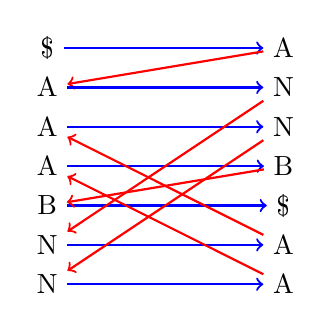
\begin{tikzpicture}
        % Horizontal distance = vertical height = 6 units
        \def\hsep{3}
        
        % Left column (top to bottom)
        \node (l1) at (0,3) {\$};
        \node (l2) at (0,2.5) {A};
        \node (l3) at (0,2) {A};
        \node (l4) at (0,1.5) {A};
        \node (l5) at (0,1) {B};
        \node (l6) at (0,.5) {N};
        \node (l7) at (0,0) {N};
        
        % Right column (top to bottom)
        \node (r1) at (\hsep,3) {A};
        \node (r2) at (\hsep,2.5) {N};
        \node (r3) at (\hsep,2) {N};
        \node (r4) at (\hsep,1.5) {B};
        \node (r5) at (\hsep,1) {\$};
        \node (r6) at (\hsep,.5) {A};
        \node (r7) at (\hsep,0) {A};
        \pause
        \draw[->, blue, thick] (l1) -- (r1);
        \pause 
        \draw[->, red, thick] (r1) -- (l2); % $ -> U
        \pause
        \draw[->, blue, thick] (l2) -- (r2); % 
        \pause
        % L-> R
        ; % 
        \draw[->, blue, thick] (l3) -- (r3); % 
        \draw[->, blue, thick] (l4) -- (r4); % 
        \draw[->, blue, thick] (l5) -- (r5); % 
        \draw[->, blue, thick] (l6) -- (r6); % 
        \draw[->, blue, thick] (l7) -- (r7); % 
        
        % Arrows from right to left (originally green, now blue)
        \draw[->, red, thick] (r2) -- (l6); % A -> V
        \draw[->, red, thick] (r3) -- (l7); % A -> $
        \draw[->, red, thick] (r4) -- (l5); % A -> B
        % \draw[->, red, thick] (r5) -- (l3); % B -> N
        \draw[->, red, thick] (r6) -- (l3); % N -> N
        \draw[->, red, thick] (r7) -- (l4); % N -> A

        \end{tikzpicture}
        \end{center}
    % \pause
    % follow the tip of blue arrows to get back the initial message: \texttt{BANANA\$}
\end{frame}


    \end{document}